\section{One Variable Integral Calculus}

\subsection{The Mercator Map and the Integral of Secant}

\subsubsection*{Historical Motivation}

The Mercator Map of the world spaces out the lines of latitude in a particular way inorder to solve a problem in naval navigation. 
The problem is that ships would navigate by sailing with a fixed angle to due north (e.g. as seen on a compass). 
This creates an issue for making map. 
Consider a map where the lines of latitude are spaced out evenly in the vertical direction (so NOT the Mercator map); for such a map, a course with fixed angle to magnetic north is NOT a straight line on the map.  
The figure below shows the path of a course with constant angle to magnetic north on a map with uniformly spaced lines of latitude.

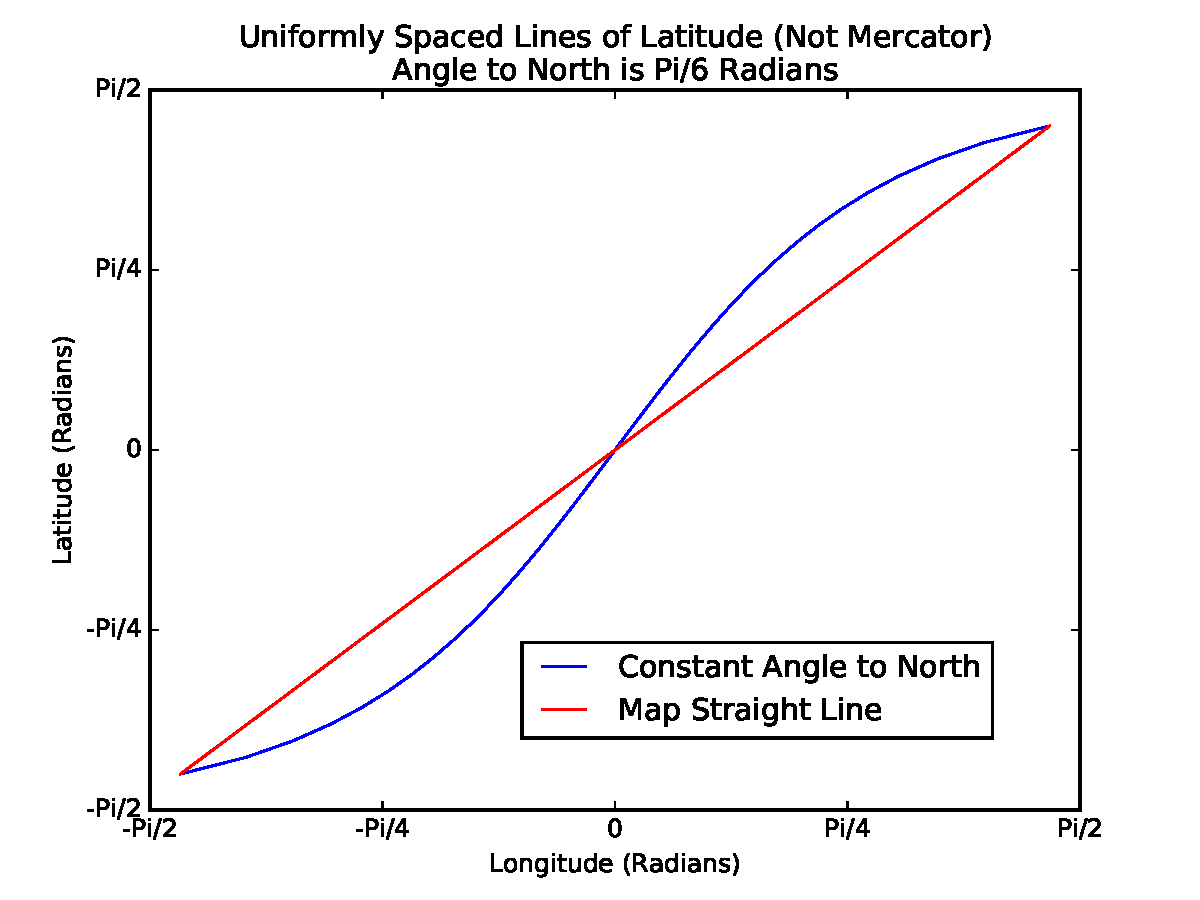
\includegraphics[width = 5in]{oneVarIntCalc/nonMercator.pdf}

The problem is that the lines of latitude get represent shorter and shorter distances as you move from the equator towards either of the poles. 
This means that there is a complicated relationship between the angle measured on this map and the true angle to magnetic north it represents.

In 1569, Mercator had the idea that he could create a map where the lines of latitude are NOT spaced evenly; if you choose the variation in spacing in the correct manner, then a course with fixed angle to magnetic north will be a straight line on this new map. 
Furthermore, the angle measured on the map will match the true angle to magnetic north.
Consider the following figure that shows a course with constant angle to magnetic north on a Mercator map, note that the lines of latitude are not evenly spaced (the values marked are multiples of \(\pi/9\) radians).

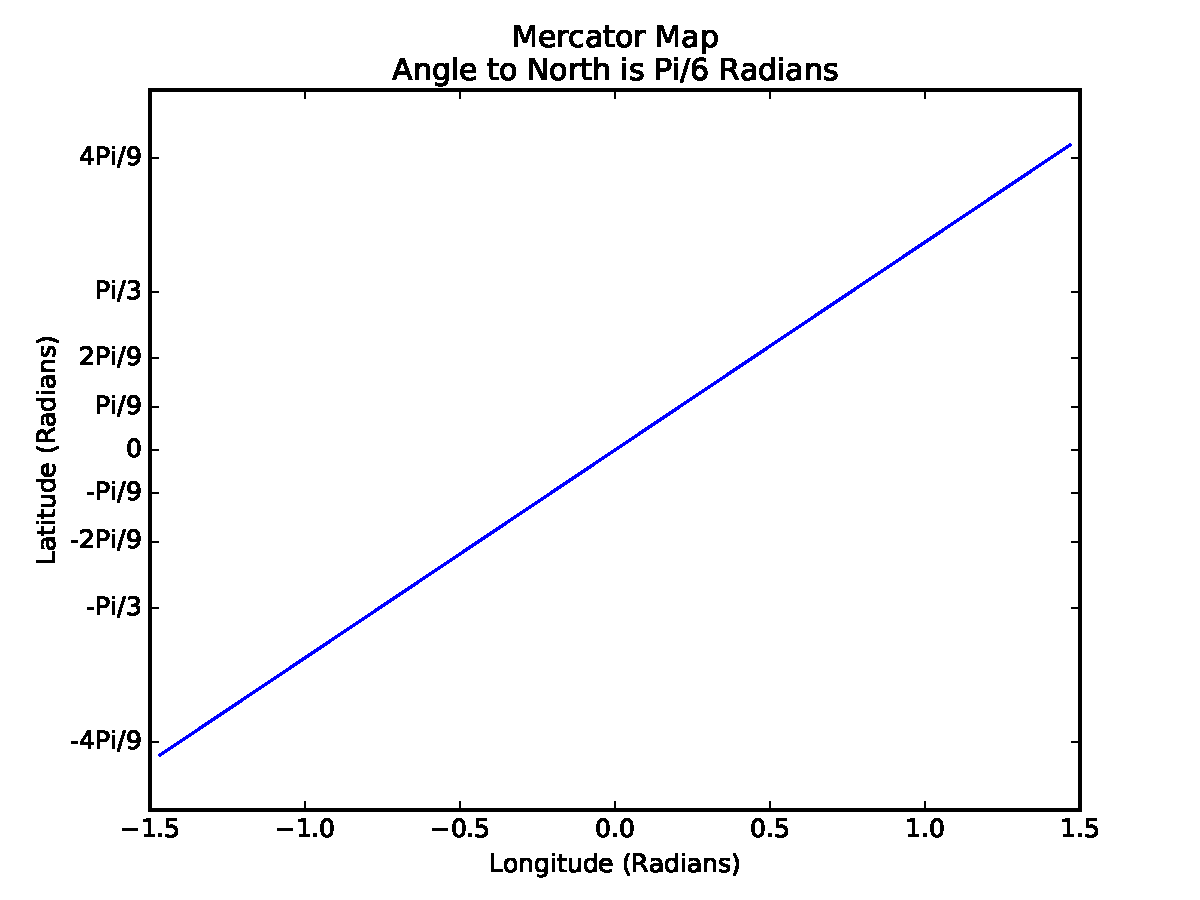
\includegraphics[width = 5in]{oneVarIntCalc/mercator.pdf}

Unfortunately, Mercator didn't give a clear formula to precisely describe how to space out the lines of latitude. 
However, in 1599, Edward Wright found a precise mathematical description of how to space out the lines; he found that the spacing depended on the area under the secant function.
He didn't know how to precisely compute this area, but he was able to approximate it. 

Later in the 1640's, Henry Bond looked at a table of these approximate areas and a table of logarithms of trigonometic functions. 
He noticed a similarity in the two tables, and he was able to conjecture a precise formula for the area under the secant function. 
We now know that his conjecture was correct, but at the time there was no proof beyond numerical tables.

A proof was later given by Isaac Barrow; this proof is the earliest known publication of the use of integration by partial fractions.

\subsubsection*{The Problem}

Compute the integral
\begin{equation}
\int\limits_0^x \sec(u) \du.
\end{equation}

\subsubsection*{The Solution}

Recall that \(\sec(u) = \frac{1}{\cos(u)}\). First, let's use algebraic manipulation combined with the trigonometric formula \(\cos^2(u) + \sin^2(u) = 1\).
\begin{align}
\int\limits_0^x \frac{1}{\cos(u)} \du & = \int\limits_0^x \frac{\cos(u)}{\cos^2(u)} \du, \\
    & = \int\limits_0^x \frac{\cos(u)}{1 - \sin^2(u)} \du.
\end{align}

Now, we do a \(u\)-substitution. However, we are already use the variable \(u\), so let's make it a "\(w\)-substitution". 
We use \(w = \sin(u)\), and so \(\dw = \cos(u) \du\). Then we have that our integral is:
\begin{equation}
\int\limits_0^{\sin(x)} \frac{1}{1 - w^2} \dw.
\end{equation}
 Now, we use partial fractions: 
\begin{align}
\frac{1}{1 - w^2} & = \frac{1}{(1 - w)(1 + w)},\\
    & = \frac{A}{1 - w} + \frac{B}{1 + w}.
\end{align}

Combining terms and comparing numerators, we get \(A + B + (A - B)w = 1\). So we have
\begin{equation}
\begin{cases}
A + B = 1, \\
A - B = 0.
\end{cases}
\end{equation}
Solving we get \(A = B = \frac{1}{2}\).

Therefore, our integral becomes
\begin{align}
\int\limits_0^{\sin(x)} \frac{1}{2(1 - w)} + \frac{1}{2(1 + w)} \dw 
    & = \left. \frac{1}{2} \log\left(\frac{1 + w}{1 - w}\right)\right|_0^{\sin(x)}, \\
    & = \frac{1}{2} \log\left(\frac{1 + \sin(x)}{1 - \sin(x)}\right).
\end{align}

To simplify things, we can now use some trigonometric identities.
\begin{align}
\frac{1}{2} \log\left(\frac{1 + \sin(x)}{1 - \sin(x)}\right) & = \log\sqrt{\frac{1 + \sin(x)}{1 - \sin(x)}}, \\
    & = \log\sqrt{\frac{(1 + \sin(x))^2}{1 - \sin^2(x)}}, \\
    & = \log\left(\frac{1 + \sin(x)}{\cos(x)}\right), \\
    & = \log(\sec(x) + \tan(x)).
\end{align}
